
% Copyright (c) 2015 - 2019 Mario Mlačak, mmlacak@gmail.com
% Licensed and published as Public Domain work.

% Age of Aquarius chapter =============================================
\chapter*{Age of Aquarius}
\addcontentsline{toc}{chapter}{Age of Aquarius}

\begin{flushright}
\parbox{0.8\textwidth}{
\emph{The greatest difficulty with the world is not its ability to produce, but the unwillingness to share. \\
\hspace*{\fill}{\textperiodcentered \textperiodcentered \textperiodcentered \hspace*{0.2em} Roy L. Smith} } }
\end{flushright}

\noindent
Age of Aquarius is chess variant which is played on 14 x 14 board,
with light yellow and light green fields and light tan-gold and
dark green pieces. In algebraic notation, columns are enumerated
from 'a' to 'n', and rows are enumerated from '1' to '14'. A new
piece is introduced, Unicorn.

\clearpage % ..........................................................
% Unicorn *************************************************************

\section*{Unicorn}
\addcontentsline{toc}{section}{Unicorn}

\noindent
\begin{wrapfigure}[7]{l}{0.4\textwidth}
\centering
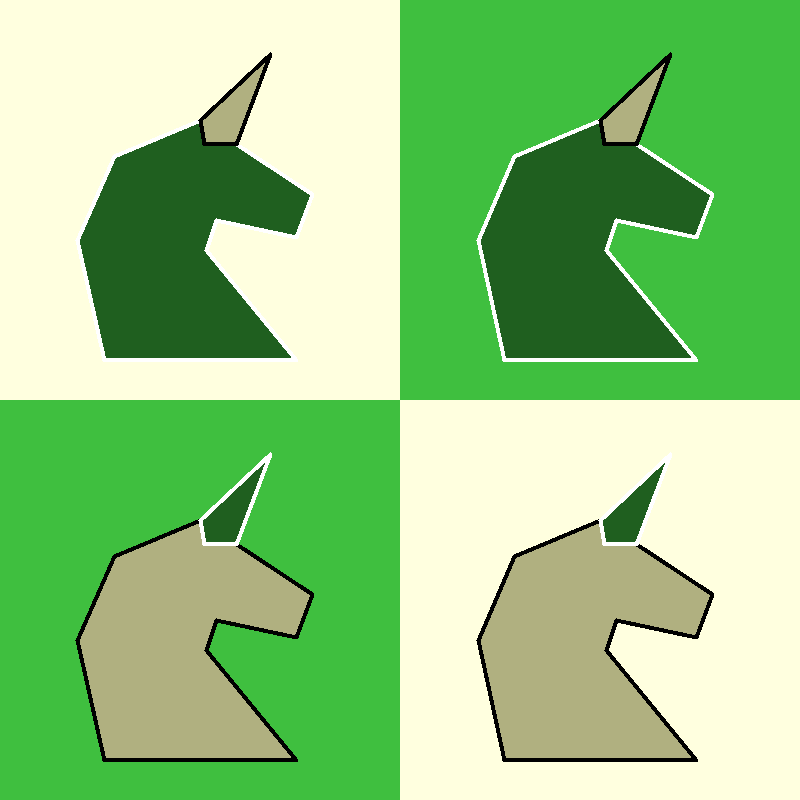
\includegraphics[width=0.4\textwidth, keepaspectratio=true]{pieces/09_unicorn.png}
\caption{Unicorn}
\label{fig:09_unicorn}
\end{wrapfigure}
Unicorn is a piece similar to Knight, only it can jump longer on
opposite color fields. Just as Knight, Unicorn is not obstructed
by any piece in its' surroundings.

In algebraic notation, symbol for Unicorn is 'U'.

\vspace{4\baselineskip}
\subsection*{Movement}
\addcontentsline{toc}{subsection}{Movement}
\label{sec:Age of Aquarius/Unicorn/Movement}

\noindent
\begin{wrapfigure}{l}{0.4\textwidth}
\centering
\includegraphics[width=0.4\textwidth, keepaspectratio=true]{examples/08_aoa/scn_aoa_01_unicorn_same_color.png}
\caption{Unicorn short jump}
\label{fig:scn_aoa_01_unicorn_same_color}
\end{wrapfigure}
On fields with the same color as Unicorn, it can move exactly the
same way Knight does.

\clearpage % ..........................................................

\noindent
\begin{figure}[!h]
% \begin{figure}[!t]
\includegraphics[width=1.0\textwidth, keepaspectratio=true]{examples/08_aoa/scn_aoa_02_unicorn_opposite_color.png}
\caption{Unicorn long jump}
\label{fig:scn_aoa_02_unicorn_opposite_color}
% \centering
\end{figure}

On fields in opposite color, Unicorn can jump much longer. Again, just as
Knight, Unicorn is not hampered by surrounding pieces. Own pieces on marked
step-fields would prevent Unicorn to move. The same marked fields are also
capture-fields, opponent's pieces on them could be captured.

For comparison, Knight's step-fields are also numbered (gray).

% ************************************************************* Unicorn
\clearpage % ..........................................................
% Promotion ***********************************************************

\section*{Promotion}
\addcontentsline{toc}{section}{Promotion}
\label{sec:Age of Aquarius/Promotion}

In all variants prior to this one promotion was forced, Pawn had to be
promoted immediately upon reaching opposite end of chessboard (or when
\hyperref[sec:Mayan Ascendancy/Pyramid/Promotion]{reached by own Pyramid} on
\hyperref[sec:Definitions/Sides of chessboard]{opponent's side of the board}).
Promotion otherwise is identical to one in Classical Chess, which is
described in details here: \\
\href{https://en.wikipedia.org/wiki/Promotion\_(chess)}{https://en.wikipedia.org/wiki/Promotion\_(chess)}.

In this variant promotion is not forced, Pawn does not have to be promoted
immediately, or at all. Pawn can be promoted later in a game, if it hasn't
moved between being tagged for promotion and actual promotion itself. Thus,
promotion can take place only on a field at which Pawn has been tagged for
promotion.

If tagged Pawn moves before actual promotion, that opportunity has been
lost. Field at which Pawn has been tagged for promotion does not hold tag,
and does not grant ability to promote to any other Pawn passing over it.

Delayed promotion is a complete move, it can contain only promotion of one
Pawn and nothing else.

\clearpage % ..........................................................

\noindent
% \begin{figure}[t]
\begin{figure}[h]
\includegraphics[width=1.0\textwidth, keepaspectratio=true]{examples/08_aoa/scn_aoa_03_delayed_promo_init.png}
\caption{Promotion start}
\label{fig:scn_aoa_03_delayed_promo_init}
% \centering
\end{figure}

Here, light player is about to tag Pawn 2 for promotion, using Pyramid
activated by Bishop. Note, Pawn 3 is not yet eligible for promotion, as it's
still on own side of chessboard.

\clearpage % ..........................................................

\noindent
% \begin{figure}[t]
\begin{figure}[h]
\includegraphics[width=1.0\textwidth, keepaspectratio=true]{examples/08_aoa/scn_aoa_04_delayed_promo_pawn_2_tagged.png}
\caption{Pawn 2 tagged for promotion}
\label{fig:scn_aoa_04_delayed_promo_pawn_2_tagged}
% \centering
\end{figure}

To speed things up, next images show dark player's response (grey arrow),
and light player's plan for next move (green arrow). Each depicted position
is after dark player's move, but before light player's move.

Here, dark Unicorn is attacking tagged Pawn 2. Pawn 2 is to move next.

\clearpage % ..........................................................

\noindent
% \begin{figure}[t]
\begin{figure}[h]
\includegraphics[width=1.0\textwidth, keepaspectratio=true]{examples/08_aoa/scn_aoa_05_delayed_promo_pawn_2_moved.png}
\caption{Pawn 1 about to get promotion}
\label{fig:scn_aoa_05_delayed_promo_pawn_2_moved}
% \centering
\end{figure}

Dark Unicorn closed in, attacking both Pawn 2 and Bishop. Since Pawn 2 moved
away from field P at which it was tagged for promotion, that opportunity has
been lost, and can't be recovered. Label P on a field just marks where Pawn 2
was tagged for promotion. Field P isn't special in any way, it won't make e.g.
Pawn 3 tagged for promotion when reached.

Light Pawn 1 is about to go next.

\clearpage % ..........................................................

\noindent
% \begin{figure}[t]
\begin{figure}[h]
\includegraphics[width=1.0\textwidth, keepaspectratio=true]{examples/08_aoa/scn_aoa_06_delayed_promo_pawn_1_tagged.png}
\caption{Pawn 1 tagged for promotion}
\label{fig:scn_aoa_06_delayed_promo_pawn_1_tagged}
% \centering
\end{figure}

Light Pawn 1 is now tagged for promotion, and is to be promoted later.
Dark Unicorn closed in again, capturing light Bishop.

Light Pawn 2 is about to go next.

\clearpage % ..........................................................

\noindent
% \begin{figure}[t]
\begin{figure}[h]
\includegraphics[width=1.0\textwidth, keepaspectratio=true]{examples/08_aoa/scn_aoa_07_delayed_promo_pawn_1_promoted.png}
\caption{Pawn 1 promoted}
\label{fig:scn_aoa_07_delayed_promo_pawn_1_promoted}
% \centering
\end{figure}

Dark Unicorn captures light Pawn 2.

Light Pawn 1 is promoted to Queen.

\clearpage % ..........................................................
% Converting tagged Pawn ----------------------------------------------

\subsection*{Converting tagged Pawn}
\addcontentsline{toc}{subsection}{Converting tagged Pawn}

Converting opponent's Pawns tagged for promotion in own Pawn or figure row
grants them ability to be rushed, and subjects them to opponent's en passant
move.

\noindent
% \begin{figure}[t]
\begin{figure}[h]
\includegraphics[width=1.0\textwidth, keepaspectratio=true]{examples/08_aoa/scn_aoa_11_tagged_pawn_conv_init.png}
\caption{Dark Pawns to be tagged}
\label{fig:scn_aoa_11_tagged_pawn_conv_init}
% \centering
\end{figure}

This example contains 3 situations, which would be driven in paralel, to speed
things up a bit.

\clearpage % ..........................................................

\noindent
% \begin{figure}[t]
\begin{figure}[h]
\includegraphics[width=1.0\textwidth, keepaspectratio=true]{examples/08_aoa/scn_aoa_12_tagged_pawn_conv_tagged.png}
\caption{Dark Pawns to be converted}
\label{fig:scn_aoa_12_tagged_pawn_conv_tagged}
% \centering
\end{figure}

Now, all dark Pawns tagged for promotion are getting converted.

Normally, Pawn gets promoted right away, because it saves move and makes better
figure available immediately. That might allow opponent to convert e.g. a Queen.
By just tagging a Pawn, it makes a latent threat, without overwhelming gains.

\clearpage % ..........................................................

\noindent
% \begin{figure}[t]
\begin{figure}[h]
\includegraphics[width=1.0\textwidth, keepaspectratio=true]{examples/08_aoa/scn_aoa_13_tagged_pawn_converted.png}
\caption{Rushing converted Pawn}
\label{fig:scn_aoa_13_tagged_pawn_converted}
% \centering
\end{figure}

Converted Pawns 1 and 3 can now be rushed, up to (and including) the row
reachable by ordinary Pawn 4. Note, Pawn 2 can't be rushed as it has been
convered outside of piece rows.

As with ordinary rush, rushing converted Pawns can only be performed as Pawn's
initial move. For instance, if Pawn 3 first moves to Pawn row (i.e. 1 field
forward), it loses opportunity to rush.

Generaly, all Pawns (own or converted) can be rushed up to the (and including)
furthest own row of chessboard, i.e. after rush they still have to reside on
\hyperref[sec:Definitions/Sides of chessboard]{own side of the board}.
Pawns can only be rushed from Pawn and figure rows.

\subsection*{Figure, Pawn, piece and rush rows}
\addcontentsline{toc}{subsection}{Figure, Pawn, piece and rush rows}
\label{sec:Age of Aquarius/Promotion/Figure, Pawn, piece and rush rows}

Figure, Pawn and piece rows refer to rows with corresponding content on initial
setup of chessboard.

Piece row is either Pawn row or figure row.

Rush row is any row from which Pawn can be rushed. Rush rows are the same as
piece rows.

\clearpage % ..........................................................

\noindent
% \begin{figure}[t]
\begin{figure}[h]
\includegraphics[width=1.0\textwidth, keepaspectratio=true]{examples/08_aoa/scn_aoa_14_pawn_figure_piece_rush_rows.png}
\caption{Pawn and figure rows}
\label{fig:scn_aoa_14_pawn_figure_piece_rush_rows}
% \centering
\end{figure}

So, Pawn rows are marked blue and red. Figure rows are marked green and grey.
Piece rows are all marked rows, and are the same as rush rows.

% ---------------------------------------------- Converting tagged Pawn
% *********************************************************** Promotion
\clearpage % ..........................................................

\section*{En passant}
\addcontentsline{toc}{section}{En passant}

\noindent
\begin{wrapfigure}{l}{0.4\textwidth}
\centering
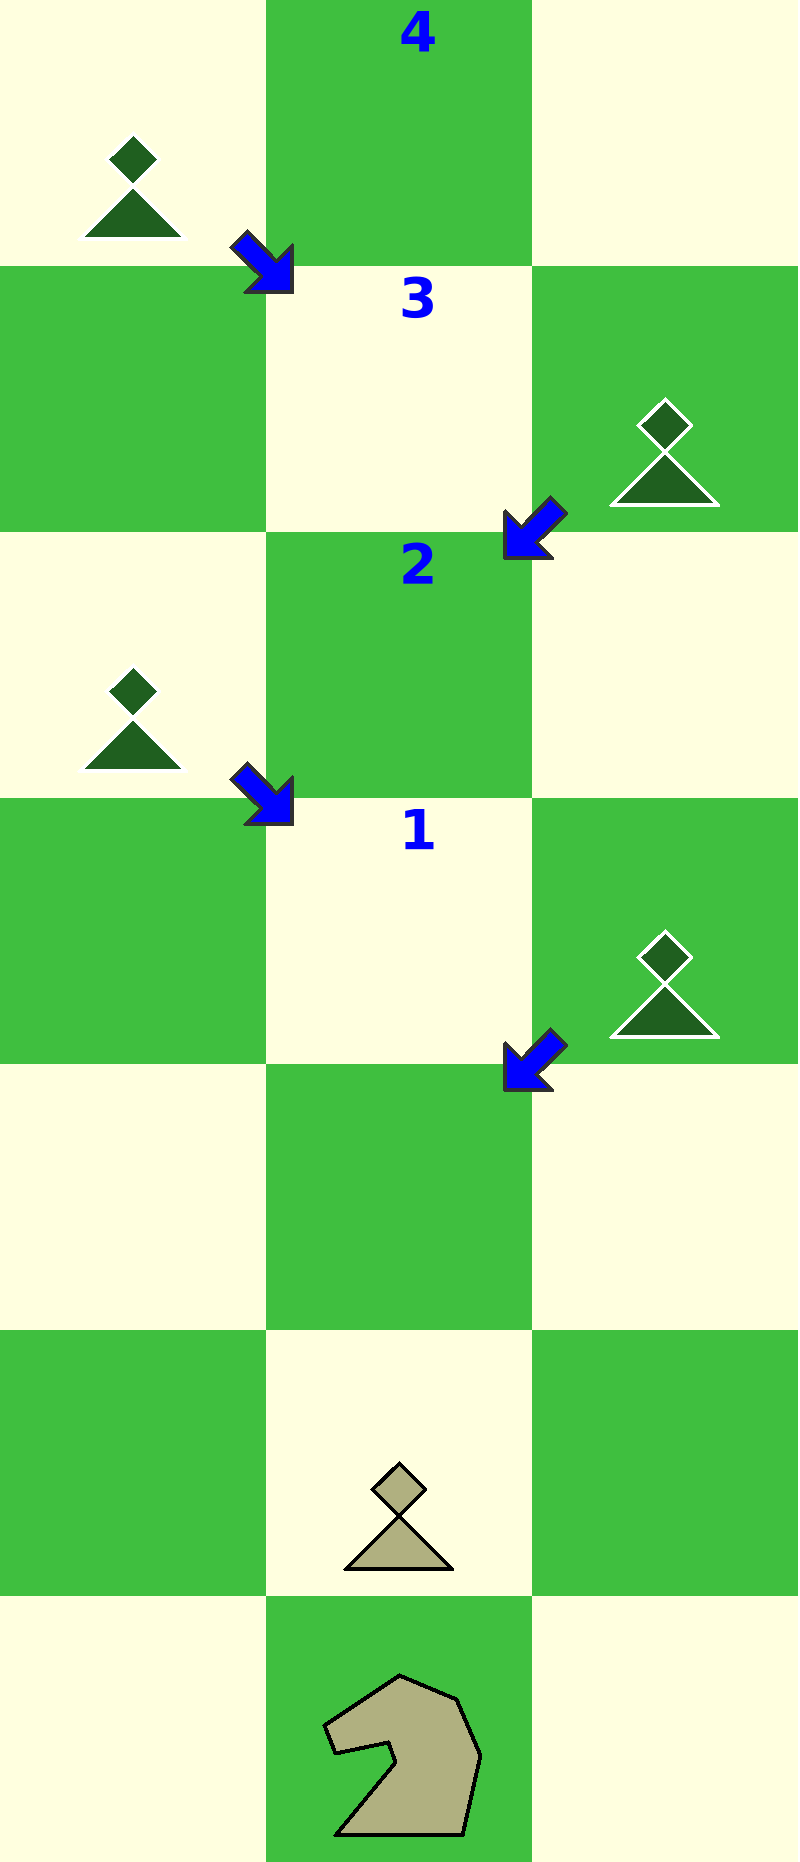
\includegraphics[width=0.214285714286\textwidth, keepaspectratio=true]{en_passants/08_age_of_aquarius_en_passant.png}
\caption{En passant}
\label{fig:08_age_of_aquarius_en_passant}
\end{wrapfigure}
Rush and en passant are identical to those in Classic Chess, only difference
is that Pawn can now move longer on initial turn, up to 5 fields in this
variant.

\clearpage % ..........................................................

\section*{Castling}
\addcontentsline{toc}{section}{Castling}

Castling is the same as in Classical Chess, only difference is that King can move 2, 3, 4 or 5 fields across.
All other constraints from Classical Chess still applies.

\noindent
\begin{figure}[!h]
% \begin{figure}[!t]
\includegraphics[width=1.0\textwidth, keepaspectratio=true]{castlings/08_aoa/age_of_aquarius_castling.png}
\caption{Castling}
\label{fig:age_of_aquarius_castling}
% \centering
\end{figure}

In example above, all valid King's castling moves are numbered.

\noindent
\begin{figure}[!h]
% \begin{figure}[!t]
\includegraphics[width=1.0\textwidth, keepaspectratio=true]{castlings/08_aoa/age_of_aquarius_castling_left_04.png}
\caption{Castling long left}
\label{fig:age_of_aquarius_castling_left_04}
% \centering
\end{figure}

In this example King was castling long to the left. Initial King's position is marked with "K".
After castling is finished, left Rook ends up on the field immediately right to the King.

\clearpage % ..........................................................

\section*{Initial setup}
\addcontentsline{toc}{section}{Initial setup}

Compared to initial setup of Mayan Ascendancy, Unicorn is inserted between Pyramid and Knight
symmetrically, on both sides of chessboard. This can be seen in the image below:

\noindent
% \begin{figure}[t]
\begin{figure}[h]
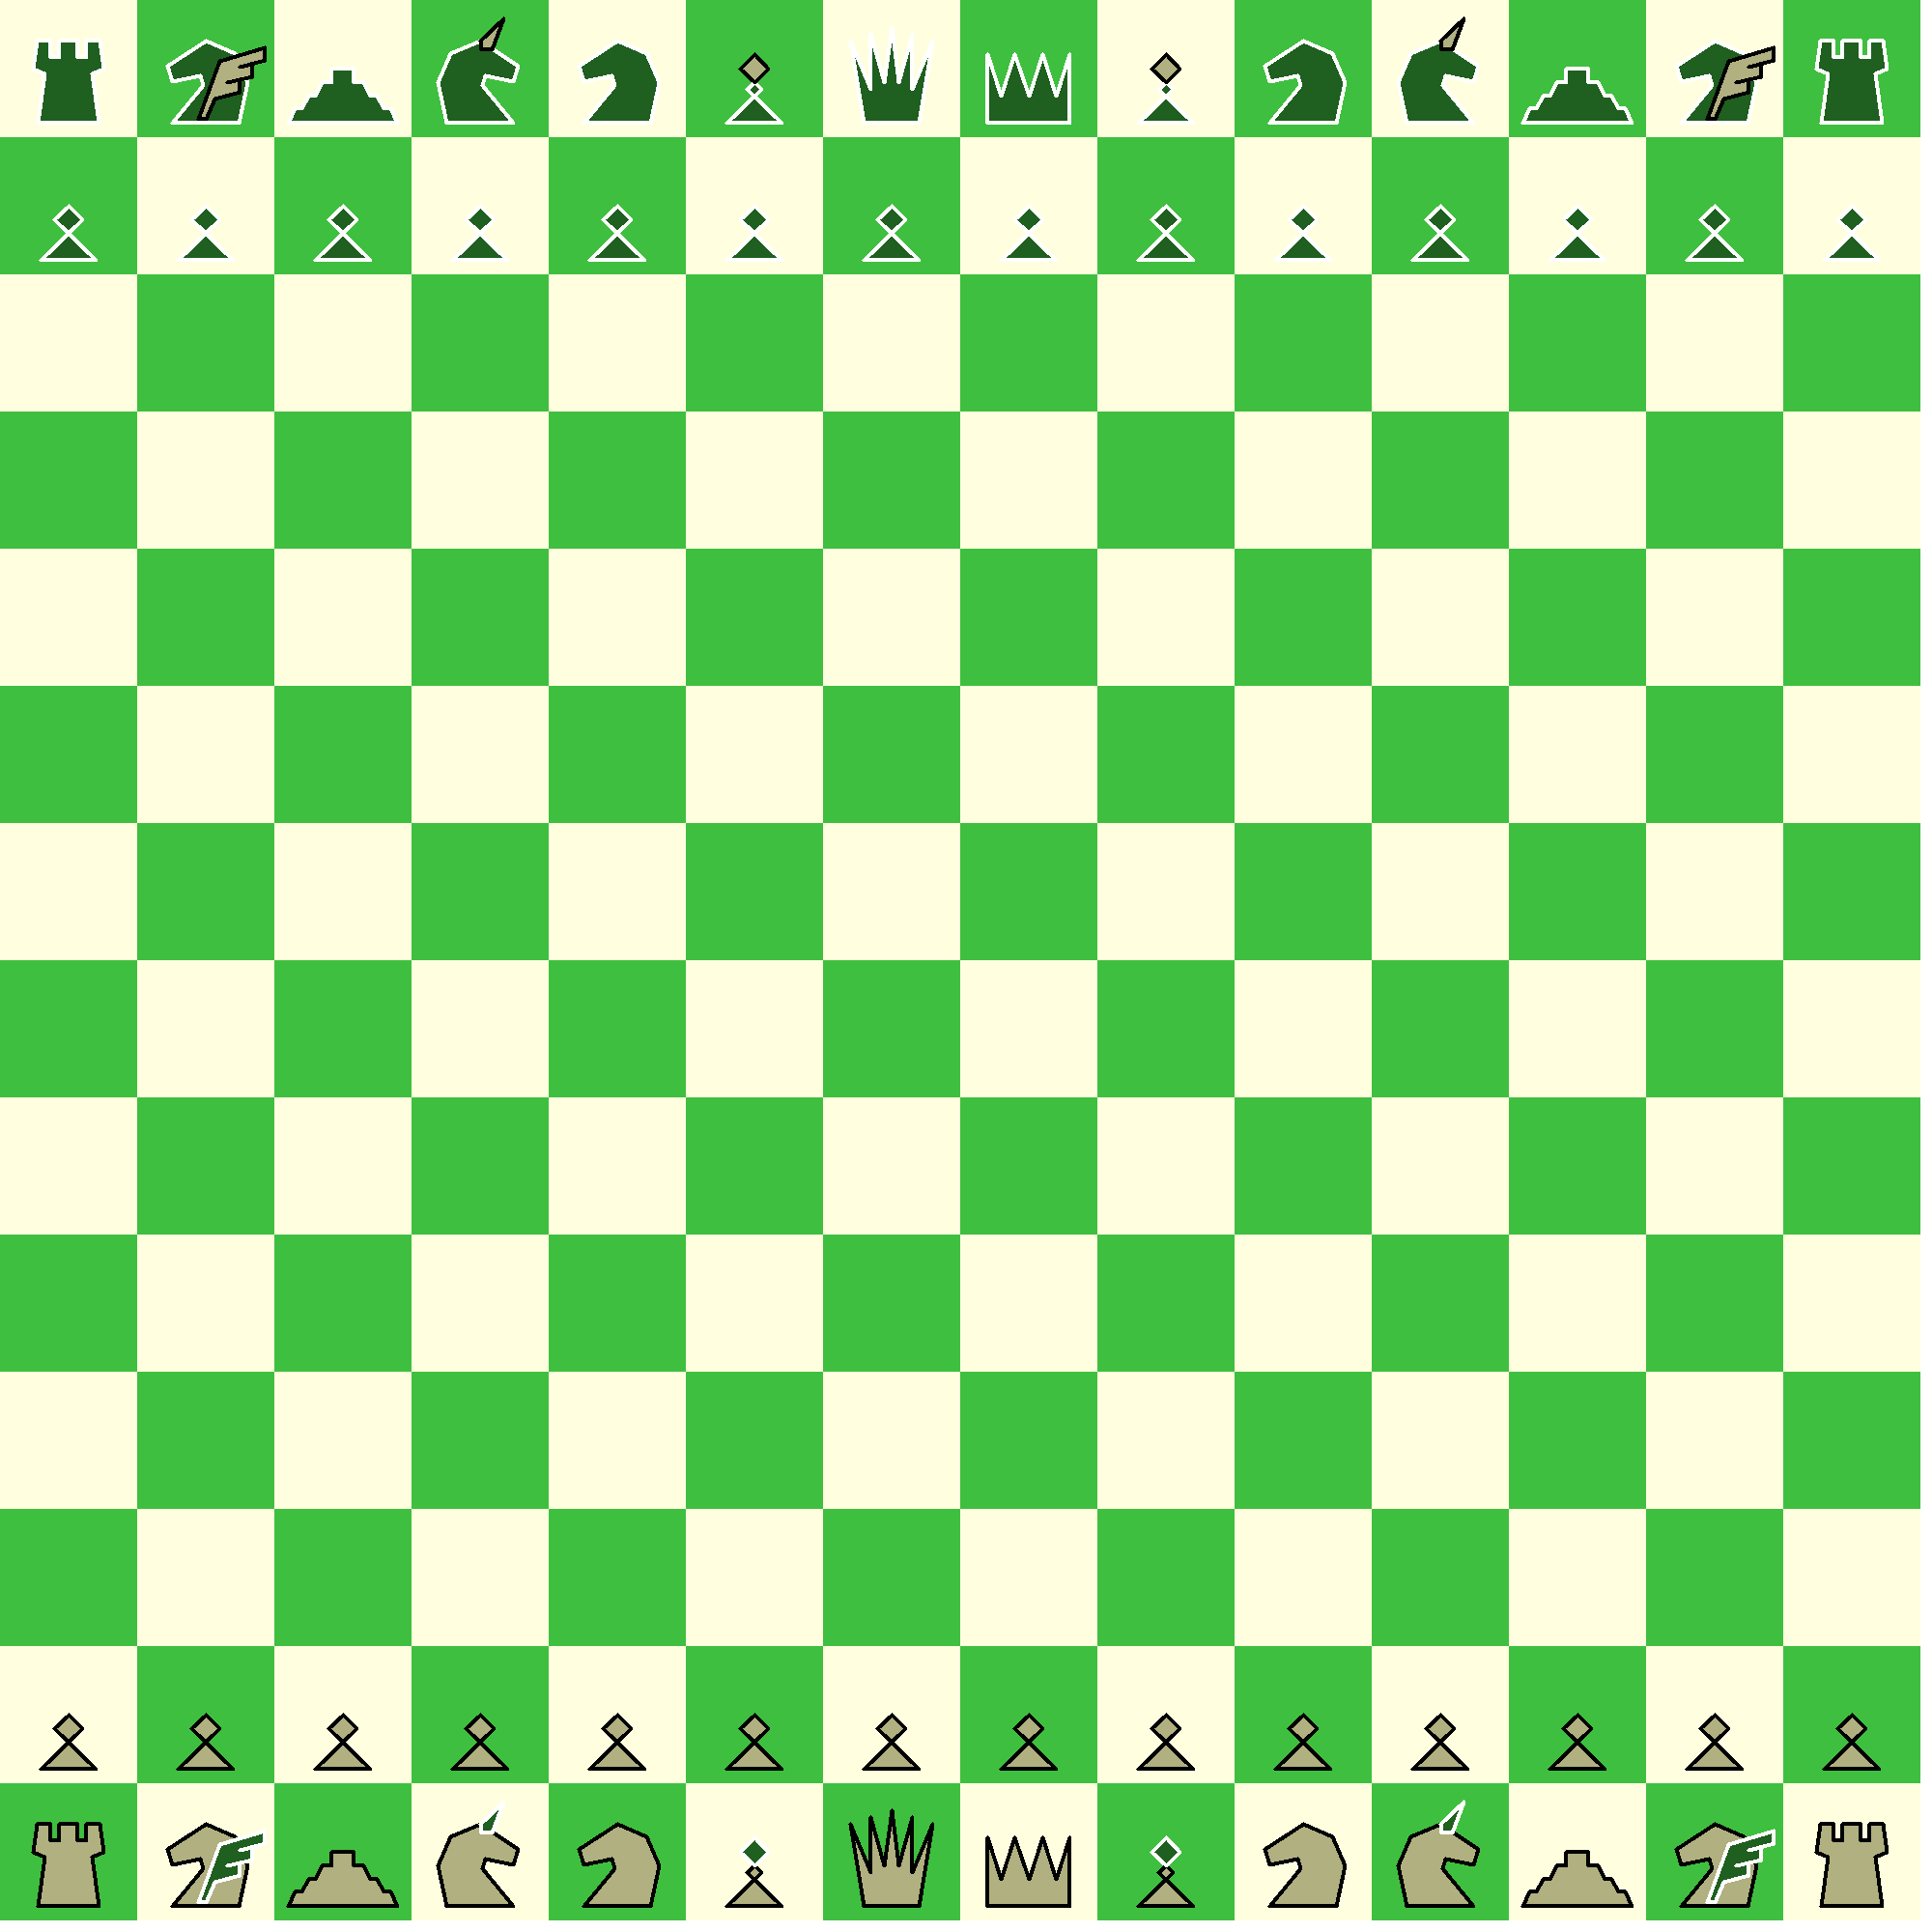
\includegraphics[width=1.0\textwidth, keepaspectratio=true]{boards/08_age_of_aquarius.png}
\caption{Age of Aquarius board}
\label{fig:08_age_of_aquarius}
% \centering
\end{figure}

\clearpage % ..........................................................
% ============================================= Age of Aquarius chapter
